\documentclass[11pt]{ltjsarticle}
\usepackage{amsmath,ascmac,amssymb,siunitx,physics,cancel}
\usepackage[math-style=ISO,bold-style=ISO]{unicode-math}
\usepackage{graphicx,float,subcaption}
\graphicspath{{../images/}}
%% tcolorbox %%
\usepackage[svgnames]{xcolor}
\usepackage{tcolorbox}
\tcbuselibrary{skins,theorems}
\tcbset{
    enhanced,
    frame hidden,
    colback=Teal!10,
}

% hyperref %
\usepackage{hyperref}
\hypersetup{
    unicode,
    setpagesize=false,
    bookmarksnumbered=true,
    bookmarksopen=true,
    colorlinks=true,
    linkcolor=DarkCyan!80!black,
    citecolor=Chocolate,
    urlcolor=Chocolate
}

%% options %%
\renewcommand*\abstractname{}
\renewcommand{\headfont}{\bfseries}
\numberwithin{equation}{section}
\usepackage{short-commands}
\usepackage{subfiles}

\begin{document}
%%%%%%%%%%%%%%%%%%%%%%%%%%%%%%%%%%%%%%%%%%%%%%%%%%
\title{Korteweg-de Vries方程式と逆散乱法}
\author{Physics Lab. 2023 数理物理班 政岡凜太郎}
\maketitle
%%%%%%%%%%%%%%%%%%%%%%%%%%%%%%%%%%%%%%%%%%%%%%%%%%
\tableofcontents
\newpage
\section{
    導入
}
% 物理学の方程式には、線形偏微分方程式がよく現れる。
% 線形な方程式は解の線型結合をとってもまた解になるという良い性質があるため、方程式を系統的に解くことが可能である。
% Maxwell方程式やSchr\"odinger方程式がその例で、電磁場や波動関数の重ね合わせに対する線形性は精度良く確認されている。
% 物理学の中でも基本に近いこれらの法則が線形性をもつのは物理学の発展にとって幸運であった。
% 一方で、非線形な現象も山ほど知られている。
% しかしそのような問題は一般に厳密に解けないので、線形近似したり、数値計算に頼ったりする。

以下の非線形偏微分方程式をKorteweg–de Vries (KdV)方程式と呼ぶ。
\begin{align}\tcboxmath{
    \pdv{u}{t} = 6u\pdv{u}{x} - \pdv[3]{u}{x}
    \label{kdv-eq}
}\end{align}
$u$は$x,t$に依存する実数の2変数関数である。
この方程式は浅水波を記述する方程式の1つとして知られているが、この記事では流体力学からKdV方程式を導くようなことはせず、とにかく与えられた方程式を色々と調べてみようという立場をとる。

KdV方程式はソリトンという興味深い解をもつことが知られている。
この解は孤立した波束であり、形が崩れることなく一定の速度で運動するようなものである。
さらに、速度の異なるソリトンを重ね合わせた
\footnote{
    厳密なソリトン解を構成するためには、もちろん線形な重ね合わせではいけない。
}
初期条件を考えることで、ソリトンを衝突させることができる。
不思議なことに、ソリトンは相互作用をした後でも形を崩さず個性を保つ。
\footnote{
    KdV方程式の2-ソリトン解を以下のリンクに置いた。遊んでみると面白いかもしれない。\url{https://www.desmos.com/calculator/33f1oysw7e}
    ただし、見やすさのために$-u(x,t)$をプロットしている。
}
線形な方程式で2つの波がすり抜けるというのならわかるが、KdV方程式は非線形なのだから、ソリトンがぶつかるときの様子は単純な重ね合わせではない。しかし、少し時間を進めてやれば波はもとの綺麗なソリトンの集まりに戻っていく。
\begin{figure}[H]
    \centering
    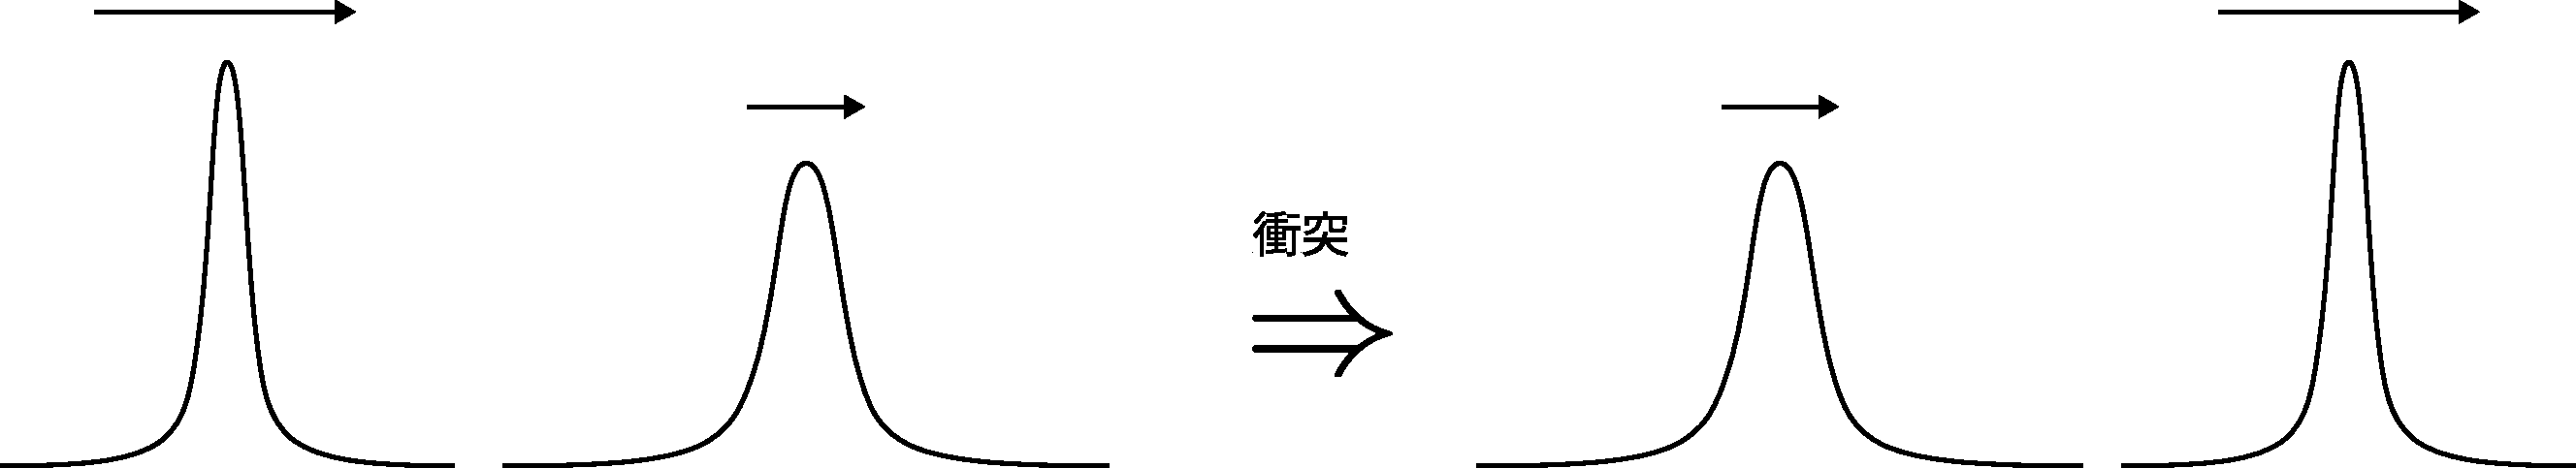
\includegraphics[width=0.8\hsize]{../images/2-soliton.pdf}
    \caption{2つのソリトンの衝突}
\end{figure}
さらに不思議なことに、初期状態をソリトンの重ね合わせにしなくとも、時間発展させれば勝手にソリトンに分かれてしまうという現象が広く見られる。
つまり、ソリトンというのはKdV方程式の解の中でありふれた構造であり、その裏に何かありそうである。
\begin{figure}[H]
    \centering
    \begin{tabular}{ccc}
    \begin{minipage}[b]{0.33\hsize}
        \includegraphics[width=\hsize]{../images/kdv_0.png}
    \end{minipage}
    &
    \begin{minipage}[b]{0.33\hsize}
        \includegraphics[width=\hsize]{../images/kdv_1.png}
    \end{minipage}
    &
    \begin{minipage}[b]{0.33\hsize}
        \includegraphics[width=\hsize]{../images/kdv_2.png}
    \end{minipage}
    \end{tabular}
    \caption{
    KdV方程式のシミュレーション結果。
    ただし、見やすさのために$-u(x,t)$をプロットしている。
    適当に与えた初期条件から勝手にソリトンに分裂していく様子が見られる。
    プログラムは\url{http://www.physics.okayama-u.ac.jp/~otsuki/lecture/CompPhys2/pde/kdv.html}を参考にした。
    }
\end{figure}

またKdV方程式は他の多くの非線形偏微分方程式と違って、初期値問題を厳密に解く方法が存在するという著しい特徴をもっている。
この解法は逆散乱法と呼ばれていて、その鍵は非線形な方程式の裏に隠れた線形な問題を見抜くことにある。
KdV方程式の場合、裏に隠れているのは量子力学でもお馴染みのSchr\"odinger方程式である。
水面波の問題を考えていたのに量子力学が現れてくる、というのはなんだか素敵ではないだろうか。

% 私がこの方程式を始めて見た時の第一印象は、「適当に非線形項を加えた汚い方程式」だった。
% この方程式の解法を勉強してその印象は払拭された。KdV方程式の各項はある必然性をもっている。
% \footnote{
% $t, x, u$のスケール変換によって、各項の係数は自由に変えることができるので、$6$や$-1$という係数は慣習的なものである。
% }
この記事の目標の1つ目は、KdV方程式が好き勝手に非線形項を加えた汚い方程式ではなく、隠れた構造を備えた方程式であると説明することである。
もっともこの記事で扱う内容は表層であり、より深い数理については\cite{Nakamura}など専門的な文献を参照してほしい。
% それから可積分な偏微分方程式はKdV方程式だけでなく、他にもたくさん(無限に)存在する。
% そのうち物理の応用の観点から見ても重要な方程式としてnon-linear Shr\"odinger方程式があるが、これについてはFadeev-Takhtajanを参照してほしい。

2つ目の目標は、逆散乱法と呼ばれる解法を用いて具体的にKdV方程式のソリトン解を求めることである。
これは技術的な話だが、具体的な解を全く求めないというのも気持ち悪いので、一応載せている。
% 数学的な厳密性は物理屋の特権で回避した。寛大な心をもって読んでほしい。それから、参考文献を載せていないが、非公式のノートということで許してほしい。

最後におまけとして、KdV方程式が無限個の保存量をもつことを擬微分演算子を用いて示している。
このような扱いはより一般的な佐藤理論につながっている。興味のある人は\cite{Nakamura}などを参照してほしい。

\newpage
\section{
    KdV方程式のソリトン解
}
\subsection{
    1-ソリトン解
}
まず単純な形で表せる1-ソリトン解を見ておこう。
解として、進行波$u(t,x) = u(x-ct)$を仮定する。
この形を(\ref{kdv-eq})に代入して整理すると、以下の常微分方程式を得る。
\begin{align}
    u''' = 6uu' + cu'
\end{align}
これを積分すると、
\begin{align}
    u'' = 3u^2 + cu + \f{b}{2}
    \label{1-soliton 1}
\end{align}
となる。$b$は積分定数である。
さらに$2u'$を掛けて積分すると、
\begin{align}
    u'^2 = 2u^3 + cu^2 + bu + a
    \label{1-soliton 2}
\end{align}
となる。
\footnote{
    (\ref{1-soliton 2})は、Weierstrassの楕円関数が満たす微分方程式と同じである。
}
$a$は積分定数である。

$u$が$|x| → ∞$で十分速く$0$に収束すると仮定すると、(\ref{1-soliton 1})、(\ref{1-soliton 2})から$b = 0,~ a = 0$となる。したがって、$u(x)$の満たす方程式は、
\begin{align}
    u'^2 = 2u^3 + cu^2
    \label{1-soliton u}
\end{align}
となる。この方程式には以下の1-ソリトン解が存在することが簡単に確認できる。
\footnote{
    $u(x)$を微分すると、
    \begin{align}
        u'(x) = -c \sech^{3}\Q(\f{\√{c}}{2}x) \cdot \f{\√{c}}{2}\sinh(\f{\√{c}}{2}x).
    \end{align}
    したがって、
    \begin{align}
        u'(x)^2
        &
        = \f{c^3}{4} \sech^{6}\Q(\f{\√{c}}{2}x)
        \Q(\cosh^2\Q(\f{\√{c}}{2}x) - 1)
        \∅ &
        = 2u^3 + cu^2
    \end{align}
    となり、(\ref{1-soliton u})が成り立つことが分かる。
}
\begin{align}
    u(x) = -\f{c}{2}\sech^2\Q(\f{\√{c}}{2}x)
    \label{1-soliton}
\end{align}
ただし、$\sech^2 x = (\cosh x)^{-2}$である。
1-ソリトン解の高さは速度$c$に比例する。また幅は$1/\√{c}$に比例する。

% 初期状態として、高さの違う1-ソリトン解を重ね合わせたもの
% \footnote{
%     厳密なソリトン解を構成するためには、もちろん線形な重ね合わせではいけない。
% }
% を考えれば、速いソリトンが遅いソリトンに追いつくという現象が見られるだろう。
% 実は不思議な事実として、ソリトンは相互作用をした後でも、形を崩さず個性を保つ。
% 線形な方程式で2つの波がすり抜けるというのならわかるが、KdV方程式は非線形なのだから、ソリトンがぶつかるときの様子は単純な重ね合わせではなく、複雑な振る舞いを見せる。しかし時間を進めてやれば波はもとの綺麗なソリトンの集まりに戻っていく。

% さらに驚くべきことに、初期状態をソリトンの重ね合わせにしなくとも、時間発展させれば勝手にソリトンに分かれてしまうという現象が広く見られる。
% つまり、ソリトンというのはKdV方程式の解の中でありふれた構造であり、その裏に何かありそうである。
% \footnote{
%     言葉で説明するよりも、見たほうが早いだろう。\url{https://www.youtube.com/watch?v=agteGpbhEaE}
% }

% \subsection{
%     Gardner変換による保存則の導出
% }
% \begin{align}
%     u = w + ϵ w_x + ϵ^2 w^2 \label{gardner}
% \end{align}
% \begin{align}
%     &\nonumber
%     u_t - 6uu_x + u_{xxx}
%     \\ &
%     = \Q(1+ϵ\pdv{x}+2ϵ^2w)\Q\Big(w_t + (-3w^2 + 2ϵ^2w^3 + w_{xx})_x) 
%     = 0
% \end{align}
% \begin{align}
%     w_t + (-3w^2 + 2ϵ^2w^3 + w_{xx})_x = 0
% \end{align}
% $∫_{-∞}^∞ w \d{x}$が保存量であることが分かる。

\subsection{
    Lax表示
}
KdV方程式を解くにあたって、まず、天下りにうまい変換を与えることにする。
% ただし、なぜこのようなものを考えるかという理由は説明する。
% 実際には、KdV方程式をうまく解くためにLax演算子を導入するというより、Lax演算子を使ってうまく解けるように、KdV方程式が定義される。
以下のような2つの演算子を定義する。
\begin{align}\tcboxmath{
    L(t) = -∂^2 + u,\q
    B(t) = -4∂^3 + 6u∂ + 3u_x
}\end{align} 
表記について注意をすると、$∂$は$x$に関する偏微分を表す演算子とする。
また$u$と書いた場合、$u(t,x)$を左から掛ける演算子を表すことにする。$u_x$などに関しても同様である。

$L(t),B(t)$をLax対と呼ぶ。
また$L(t)$はLax演算子と呼ばれ、今の場合1次元の量子力学のHaniltonianと同じ形をしている。
$L(t), B(t)$によって、KdV方程式(\ref{kdv-eq})は
\begin{align}\tcboxmath{
    \dv{L}{t} = [B(t), L(t)]
    \label{lax-eq}
}\end{align} 
と書き換えられる。これをLax方程式と呼ぶ。また与えられた方程式を(\ref{lax-eq})のように表すことをLax表示という。
Lax表示はKdV方程式に特有のものではなく、多くの可積分系に対するLax表示が知られている。

KdV方程式とLax方程式(\ref{lax-eq})が同値であることを証明しよう。
(\ref{lax-eq})の左辺は
\begin{align*}
    \dv{L}{t} = u_t
\end{align*}
となる。つぎに右辺を計算すると、
\begin{align*}
    [B(t), L(t)]
    &
    = [-4∂^3 + 6u∂ + 3u_x, -∂^2 + u]
    \∅ &
    = -4(u_{xxx} + \cancel{3u_{xx}∂} + \bcancel{3u_x∂^2})+ 6uu_x
    \∅ &\q
    + 6(\cancel{u_{xx}∂} +\bcancel{ 2u_x∂^2})
    \∅ &\q
    + 3(u_{xxx} + \cancel{2u_{xx}∂})
    \∅ &
    = 6uu_x - u_{xxx}
\end{align*}
となる。両辺を等号で結ぶことでKdV方程式を得る。Lax方程式は演算子の等式であったが、両辺が微分演算子$∂$を含まないために、$u$に対する偏微分方程式とみなせる。

Lax方程式(\ref{lax-eq})では、$B(t)$は時間発展の生成子となっている。するとLax方程式は Hamiltonian $L(t)$の$B(t)$による時間発展を考えていることになる。
ここで、$L(0)$を対角化して
\begin{align}
    L(0)ψ(x, 0) = λ ψ(x, 0)
    \label{eq: L(t)}
\end{align}
と書く。$ψ(x, 0)$は$L(0)$の固有値$λ$の固有関数である。これを時間発展させてみよう。
$ψ(x, t)$の時間発展を記述する方程式として、
\begin{align}
    ψ(x, t) = U(t)ψ(x, 0),\q
    \dv{U(t)}{t} = B(t)U(t),\q
    U(0) = 1
    \label{eq: B psi} 
\end{align}
を課す。
すると、$ψ(x, t)$は$L(t)$の固有関数であることが示せる。

% まず、時間発展演算子$U(t)$は$B(t)$によって
% \begin{align}
%     U(t) = T\exp(∫_0^t \d{t'} B(t'))
% \end{align}
% と書ける。
(\ref{eq: L(t)})の両辺に左から$U(t)$を掛けると、
\begin{align}
    U(t)L(0)U(t)^{-1}ψ(x,t) = λ ψ(x,t).
\end{align}
となる。ここで、$U(t)L(0)U(t)^{-1}$を時間微分する。
$U(t)U(t)^{-1} = 1$を時間微分すると
\begin{align}
    \dv{t}U(t)^{-1} = - U(t)^{-1}B(t)
\end{align}
が分かるので、
\begin{align}
    \dv{t}\Q(U(t)L(0)U(t)^{-1}) = [B(t), U(t)L(t)U(t)^{-1}]
\end{align}
となる。これはLax方程式なので、初期条件$U(0)L(0)U(0)^{-1} = L(0)$から、
\begin{align}
    U(t)L(0)U(t)^{-1} = L(t)
\end{align}
となる。この両辺を$ψ(x,t)$に作用させて、
\begin{align}
    L(t)ψ(x, t) = λ ψ(x, t)
\end{align}
となる。
すなわち、$B(t)$によって時間発展する波動関数$ψ(x, t)$は、任意の時刻で$L(t)$の固有関数である。
さらに、$ψ(x,t)$に対する$L(t)$の固有値は常に$λ$で時間に依存しない。
\footnote{
    逆に$L(t)$の固有値が時間変化しない条件としてLax方程式を導ける。
}

\subsection{
    逆散乱法
}
Lax方程式が$L(t) = -∂^2 + u$の等スペクトル条件を意味することを見た。これを利用して、KdV方程式を量子力学における散乱の逆問題に置き換えることができる。この解法を逆散乱法と呼ぶ。

逆散乱法では、まず散乱データと呼ばれる量を求める。これはポテンシャル$u(x, t)$に対するスペクトルと、束縛解・散乱解の遠方での漸近的な振る舞いをまとめたものである。
実は$t = 0$での散乱データが分かれば、任意の$t$での散乱データは簡単に分かってしまう。スペクトルに関しては、これが時間変化しないことから明らかだろう。

散乱データからポテンシャル$u(x, t)$を復元するのは散乱の逆問題と呼ばれ、Gel'fand-Levitan-Marchenko方程式という積分方程式によって解かれる。求まった$u(x, t)$がKdV方程式の解となる。

\subsection{
    散乱データ
}
Schr\"odinger方程式$(-∂^2 + u(x, t))ψ(x, t) = λ ψ(x, t)$
に対し、束縛状態の固有値を$λ = -κ_n^2 ~ (n=1,…,N)$とする。
% ポテンシャルが遠方で十分速く減衰する場合
%     \footnote{$∫(1+|x|)^k|u(x)| < ∞, ~ k=0,1,2$を満たす場合}
% 、$κ_n$は有限個で、縮退はないことが知られている。
遠方での解の振る舞いは、
\begin{align}
    ψ(x, t) = \begin{cases}
        c_n(t) e^{-κ_n x} & (x → +∞),
        \\
        \~{c}_n(t) e^{κ_n x} & (x → -∞)
    \end{cases}
\end{align}
となる。また、散乱状態の固有値を$λ = k^2$とおく。散乱状態の遠方での振る舞いは、
\begin{align}
    ψ(x, t) = \begin{cases}
        e^{-ikx} + b(k, t)e^{ikx} & (x → +∞),
        \\
        a(k, t)e^{-ikx} & (x → -∞).
    \end{cases}
\end{align}
となる。散乱状態では独立な解がもう一つあるが、どちらか一方の情報だけで十分である。$κ_n, c_n(t), a(k,t), b(k,t)$からなる値の集合を散乱データと呼ぶ。

波動関数は$B(t) = -4∂^3 + 6u∂ + 3u_x$によって生成される複雑な時間発展をするが、$x → ±∞$では$B(t) ≈ -4∂^3$と近似できる。したがって、
\begin{align}
    ψ(x, t) = \begin{cases}
        e^{4κ_n^3 t} c_n(0) e^{-κ_n x} & (x → +∞),
        \\
        e^{-4κ_n^3 t}\~{c}_n(0) e^{κ_n x} & (x → -∞)
    \end{cases}
\end{align}
と書ける。すなわち$c_n(t) = e^{4κ_n^3t}$である。同様に、
\begin{align}
    ψ(x, t) = \begin{cases}
        e^{-4ik^3t}e^{-ikx} + e^{4ik^3t}b(k, 0)e^{ikx}
        & (x → +∞),
        \\
        e^{-4ik^3t}a(k, 0)e^{-ikx}
        & (x → -∞)
    \end{cases}
\end{align}
となる。位相を再定義すると、$a(k, t) = a(k, 0),~ b(k, t) = e^{8ik^3t}b(k, 0)$となる。以上の結果をまとめると、
\begin{align}\tcboxmath{
    c_n(t) = e^{4κ_n^3t}c_n(0),
    \q
    a(k,t) = a(k,0),
    \q
    b(k,t) = e^{8ik^3t}b(k,0).
    \label{scattering data}
}\end{align}

\subsection{
    ソリトン
}
任意の時刻$t$での散乱データが求まったので、逆散乱問題を解けば$u(t,x)$が求まる。
ここで具体的な計算をする前に、まず目標である$N$-ソリトン解について感覚的な説明をしておく。

束縛状態の時間発展は
\begin{align}
    ψ_n(x, t) = \begin{cases}
        c_n(0) e^{-κ_n (x-4κ_n^2 t)} & (x → +∞),
        \\
       \~{c}_n(0) e^{κ_n (x-4κ_n^2t)} & (x → -∞)
    \end{cases}
\end{align}
と表せる。したがって、$ψ_n(x, t)$は$x→±∞$では速度$4κ_n^2$をもつ。
$|x|$が大きくない領域でも、$ψ_n(x,t)$はある程度この速度にしたがって移動するだろう。
さもなければ時間を進めた時に規格化条件$⟨ψ_n|ψ_n⟩ = 1$を保つことができない。

複数の束縛状態がある場合、別々の速度で移動する$ψ_n(x,t)$は、依然として全てポテンシャル$u(t,x)$に対する固有状態でなければならない。
このため$u(x, t)$は全ての束縛状態の移動に追従しなければならず、結果的に複数のピークに分裂する。このピークがソリトンである。
\begin{figure}[H]
    \centering
    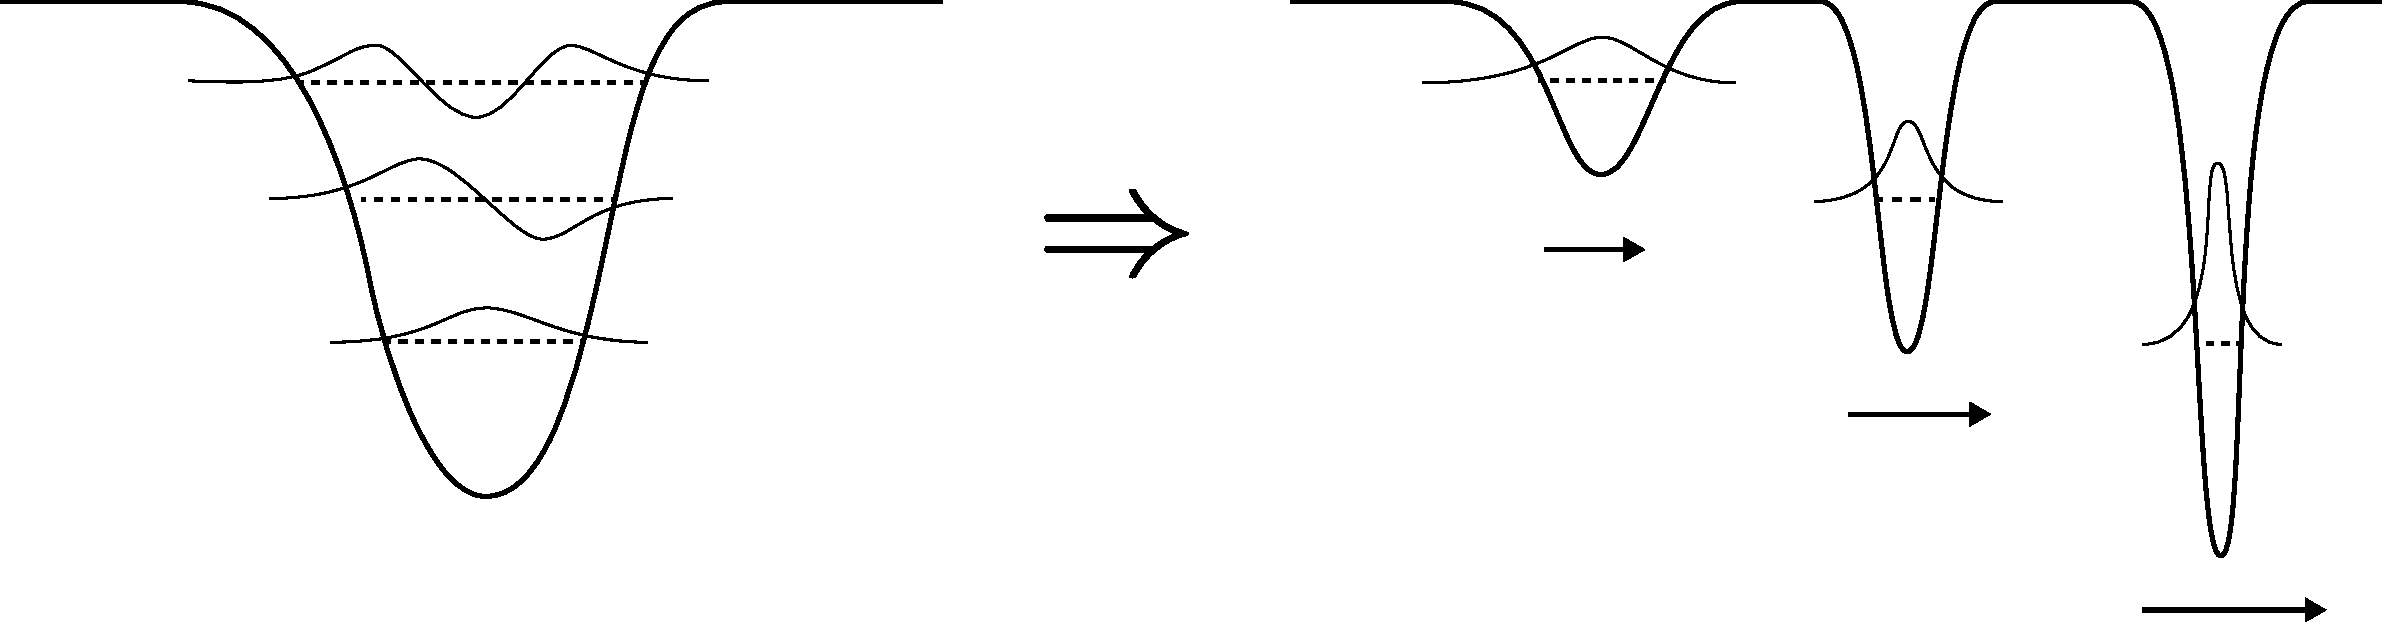
\includegraphics[width=0.7\hsize]{../images/soliton_split.pdf}
    \caption{3-ソリトン解が分裂する様子。}
\end{figure}
% 具体的には$N$-ソリトン解において
% \begin{align}
%     u(x, t) = -4 ∑_{n=1}^N κ_nψ_n(x, t)^2
% \end{align}
% と書くことができる。この式は後で示す。

以上の説明では反射係数$b(k, t)$の時間発展については触れなかった。実は$N$-ソリトン解は$b(k, t) = 0$となるような無反射ポテンシャルに対して得られる解である。反射係数の影響は、束縛状態を持たないポテンシャルのさざなみとして表れる。

\section{
    散乱の逆問題
}
この章はちょっと大変な計算パートだが、散乱データからポテンシャルを再構成すること自体が面白い問題なので、載せておいた。
\subsection{
    Jost解
}
散乱の逆問題を解くために、いくつか準備をする。
時間発展のことは一旦忘れて、時間に依存しないSchr\"odinger方程式$(-∂^2 + u(x))ψ(x) = λψ(x)$の解で、以下の条件を満たすものを考える。
\begin{align}
    f_{±}(x, k) → e^{ikx} \q (x → ±∞)
\end{align}
ただし、$λ = k^2$であり、しばらくは$k$は実数であるとする。
$f_+(x, k), f_-(x, k)$をJost解という。$f_{±}(x, k)$の複素共役をとっても解であるから、
\begin{align}
    f_{±}^*(x, k) = f_{±}(x, -k)
\end{align}
である。
また$f_{±}(x,k) = g_{±}(x,k)e^{ikx}$と定義すると、これはSchr\"odinger方程式から以下の式を満たす。
\begin{gather}
    g''_{±}(x,k) + 2ikg'_{±}(x,k) = u(x)g_{±}(x,k) \label{g_pm}
    \\
    g_{±}(x,k) → 1, \q
    g'_{±}(x,k) → 0, \q
    (x → ± ∞)
\end{gather}
(\ref{g_pm})から、
% \begin{align}
%     g''_{+}(x, k) + 2ikg'_{+}(x, k) = u(x)g_{+}(x, k)
% \end{align} 
\begin{align*}
    (e^{2ik x}g'_{+}(x,k))' = e^{2ik x}u(x)g_{+}(x,k)
\end{align*}
が成り立つ。これを$x$から$∞$まで積分して両辺に$e^{-2ikx}$を掛けると、
\begin{align*}
    -g'_{+}(x, k) = ∫_x^∞ \d{y} e^{2ik(y-x)}u(y)g_{+}(y, k)
\end{align*}
となる。さらに積分すると、
\begin{align}
    g_+(x,k) - 1
    &
    = ∫_x^∞ \d{z} ∫_z^∞ \d{y} e^{2ik(y-z)}u(y)g_+(y,k)
    \∅ &
    = ∫_x^∞ \d{y} ∫_x^y \d{z} e^{2ik(y-z)}u(y)g_+(y,k)
    \∅ &
    = ∫_x^∞ \d{y} \f{1-e^{2ik(y-x)}}{-2ik}u(y)g_+(y,k)
\end{align}
となる。
% $g_-(x, k)$についても同様の計算をすると、
% \begin{align}
%     g'_-(x, k) = ∫_{-∞}^x \d{y} e^{2ik(y-x)}u(y)g_-(y,k)
% \end{align}
% \begin{align}
%     g_-(x, k) - 1
%     &
%     = ∫_{-∞}^x \d{z} ∫_{-∞}^z \d{y} e^{2ik(y-z)}u(y)g_-(y,k)
%     \∅ &
%     = ∫_{-∞}^x \d{y} ∫_y^x \d{z} e^{2ik(y-z)}u(y)g_-(x,k)
%     \∅ &
%     = ∫_{-∞}^x \d{y} \f{e^{2ik(y-x)}-1}{-2ik}u(y)g_-(y,k)
% \end{align}
% となる。
$g_-(x,k)$についても座標を反転すれば同じことが成り立つので、
\begin{align}
    &
    g_+(x,k)
    = 1 - \f{1}{2ik} ∫_x^∞ \d{y}\Q(1-e^{2ik(y-x)})u(y)g_+(y,k),
    \\ &
    g_-(x,k)
    = 1 + \f{1}{2ik} ∫_{-∞}^x \d{y}\Q(1-e^{-2ik(x-y)})u(y)g_-(y,k)
\end{align}
が成り立つ。これらの式を逐次的に用いれば、Jost関数は$1/k$で展開された形で求めることができる。

ここで、$k$が複素数だと考える。上半平面$ℑ k > 0$において、$|k| → ∞$のとき、
\begin{align}
    &
    g_+(x,k)
    = 1 - \f{1}{2ik}∫_x^∞ \d{y} u(y) + O\Q(\f{1}{k^2})
    \label{g_+(x,k), k to infty}
    \\ &
    g_-(x,-k)
    = 1 - \f{1}{2ik}∫_{-∞}^x \d{y} u(y) + O\Q(\f{1}{k^2})
    \label{g_-(x,-k), k to infty}
\end{align}
となる。また、下半平面$ℑ k < 0$において、$|k| → ∞$のとき、
\begin{align}
    &
    g_-(x,k)
    = 1 + \f{1}{2ik}∫_{-∞}^x \d{y} u(y) + O\Q(\f{1}{k^2})
    \label{g_-(x,k), k to infty}
    \\ &
    g_+(x,-k)
    = 1 - \f{1}{2ik}∫_x^∞ \d{y} u(y) + O\Q(\f{1}{k^2})
    \label{g_+(x,-k), k to infty}
\end{align}
となる。
以上の式はJost解とポテンシャル$u(x)$を繋ぐものになっている。
ここで、$ℑk > 0$に対し、
\begin{align}\tcboxmath{
    g_+(x,k) = 1 + ∫_{-∞}^∞ \d{z} K(x,z)θ(z-x)e^{ik(z-x)}
    \label{def: K}
}\end{align}
と書く。階段関数$θ(z-x)$が掛かっているのは、物理的な解を取り出すために遅延Green関数を選択するのと同じ理由である。
つまり、$g_+(x,k)$は$x → +∞$における境界条件によって定義されるので、座標が$x$より小さい領域での散乱ポテンシャルには依存しない。
仮に$K(x,y)$が求まったとする。(\ref{def: K})を$\e^{-ikx}$について部分積分すると、$1/k$による展開が得られる。
2次まで書くと、
\begin{align}
    g_+(x,k) = 1 - \f{1}{ik}K(x,x) + O\Q(\f{1}{k^2})
\end{align}
となる。
ただし、$ℑ k > 0$を用いた。
これを(\ref{g_+(x,k), k to infty})と比べることで、
\begin{align}
    K(x, x) = \f{1}{2}∫_x^∞ \d{y} u(y)
\end{align}
を得る。ポテンシャル$u(x)$は
\begin{align}\tcboxmath{
    u(x) = -2 \dv{x}K(x,x)
    \label{u-K relation}
}\end{align}
によって求まる。
したがって$K(x,z)$を求めれば$u(x)$が求まる。
ただしそのためにはもう少し準備が必要である。

\subsection{
    反射係数・透過係数の性質
}
無限遠で以下のように振る舞う解を考えてみる。
\begin{align}
    ψ(x) ∼ \begin{cases}
        α(k)e^{-ikx} + β(k)e^{ikx}
        &
        (x → +∞)
        \\
        e^{-ikx}
        &
        (x → -∞)
        \label{psi}
    \end{cases}
\end{align}
透過係数$a(k)$と反射係数$b(k)$を以下のように定義する。
\begin{align}
    a(k) ≔ \f{1}{α(k)},
    \q
    b(k) ≔ \f{β(k)}{α(k)}
\end{align}
$ψ(x)$は$x → ±∞$でそれぞれJost解によって表せるから、
\begin{align}
    ψ(x)
    =
    α(k)f_+^*(x,k) + β(k)f_+(x,k)
    =
    f_-^*(x,k)
    \label{pm relation}
\end{align}
が成り立つ。(\ref{pm relation})とその複素共役をとった式を行列の形に書く。
\begin{align}
    \M(f_- \\ f_-^*) = \M(α^* & β^* \\ β & α)\M(f_+ \\ f_+^*)
\end{align}
ここで、Wronskian
\begin{align}
    W[f_-, f_-^*]
    = \det\M(f_- & f_-^* \\ f'_- & {f_-^*}')
    = \det\M(α^* & β^* \\ β & α) W[f_+, f_+^*]
\end{align}
を考えると、これは$x$によらない
\footnote{
    Wronskianの微分は
    \begin{align}
        \dv{x}W[f_-, f_-^*] = \det\M(f'_- & {f_-^*}' \\ f'_- & {f_-^*}') + \det\M(f_- & f^*_- \\ f''_- & {f_-^*}'')
    \end{align}
    であるが、第1項は明らかに$0$であり、第2項は$f''_- = (u-k^2)f_-,~{f_-^*}'' = (u-k^2)f^*_-$から$0$となる。
}
。一方
\begin{align}
    &
    W[f_-, f_-^*] → W[e^{ikx}, e^{-ikx}] = -2ik \q (x → -∞),
    \\ &
    W[f_+, f_+^*] → W[e^{ikx}, e^{-ikx}] = -2ik \q (x → +∞)
    \label{Wronskian ++}
\end{align}
であるから、
\begin{align}
    \det\M(α^* & β^* \\ β & α) = |α(k)|^2 - |β(k)|^2 = 1
\end{align}
が従う。これは確率の保存を意味する。透過係数・反射係数を使って書くと、
\begin{align}
    |a(k)|^2 + |b(k)|^2 = 1
\end{align}
である。
% \begin{align}
%     \M(f_+ \\ f_+^*) = \M(β & -β^* \\ -α & α^*)\M(f_- \\ f_-^*)
% \end{align}
% \begin{align}
%     α(k) = 1 - \f{1}{2ik}∫_{-∞}^{∞} \d{y}u(y) + O\Q(\f{1}{k^2})
% \end{align}
次に、$α(k)$の零点を考える。
(\ref{psi})に戻って考えてみると、$α(k) = 0$の状況は入射粒子がないにも関わらず、透過・反射が起こっているような状況である。
散乱状態ではこのようなことはありえないが、$k = iκ,~ κ > 0$と考えると、$α(k) = 0$は束縛状態の実現を意味することが分かる。このとき、
\begin{align}
    ψ(x) = f_-^*(x,\iκ) ∼ \begin{cases}
        β(iκ)e^{-κ x} & (x → +∞)
        \\
        e^{κ x} & (x → -∞)
    \end{cases}
\end{align}
となる。透過係数$a(k)$・反射係数$b(k)$は$α(k)$を分母に含むから、束縛状態は$a(k),b(k)$の極として現れることが分かる。

後の計算のために、$b(k)$の留数を求める。
これは$α(k)$の零点$k = \iκₙ$に対し$β(\iκₙ)/\.α(\iκₙ)$ (ドットは$k$微分)によって求めることができる。
$k$が実数ではない場合、もはや$f_{±}^*(x,k) = f_{±}(x,-k)$は成り立たないが、以降の議論では$f_{±}^*(x,k)$と書いたとき、記号的に$f_{±}(x,-k)$を意味することとする。
(\ref{pm relation}),(\ref{Wronskian ++})から
\begin{align}
    W[f_+, f_-^*] &= α(k)W[f_+,f_+^*]
    = -2ik α(k)
\end{align}  
が成り立つ。両辺を$k$で微分すると、
\begin{align}
    -2iα(k) - 2ik \.{α}(k) = W[\.f_+, f_-^*] + W[f_+, \.f_-^*].
\end{align}  
ただし$k$微分をドットで表した。$f_-^*(x,k)$は微分方程式
\begin{align}
    {f_-^*}''(x,k) = (u(x) - k^2)f^*_-(x,k)
\end{align}
を満たす。また$\.f_+(x,k)$は微分方程式
\begin{align}
    \.f''_+(x,k) = (u(x)-k^2)\.f_+(x,k) - 2k f_+(x,k)
\end{align}
を満たすので、
\begin{align}
    \dv{x}\det\M(\.f_+ & f_-^* \\ \.f'_+ & {f_-^*}')
    = \det\M(\.f_+ & f_-^* \\ \.f''_+ & {f_-^*}'') = 2kf_+f_-^*.
\end{align}
同様に
\begin{align}
    \dv{x}\det\M(f_+ & \.f_-^* \\ f'_+ & \.f^*_-{}')
    = \det\M(f_+ & \.f_-^* \\ f''_+ & \.f^*_-{}'')
    = -2kf_+f_-^*
\end{align}
であるから、
\begin{align}
    W[\.f_+, f_-^*]\eval_x^∞ &= 2k ∫_x^∞ \d{y} f_+(y,k)f_-^*(y,k)
    \label{Wronskian dot f_+ f_-^*}
    \\
    W[f_+^*, \.f_-]\eval_{-∞}^x &= -2k ∫_{-∞}^x \d{y} f_+(y,k)f_-^*(y,k)
    \label{Wronskian f_+^* dot f_-}
\end{align}
となる。
$α(k)$の零点$iκ_n$においては、$f_-^*(x,\iκ_n)=β(\iκ_n)f_+(x,\iκ_n)$が成り立つので、
\begin{align}
    W[\.f_+, f_-^*] = β(iκ_n) W[\.f_+, f_+],
    \q
    W[f_+, \.f_-^*] = \f{1}{β(iκ_n)} W[f_-^*, \.f_-^*]
\end{align}
となる。したがって、$W[\.f_+, f_-^*]$は$x → ∞$で$0$に収束し、$W[f_+, \.f_-^*]$は$x → -∞$で$0$に収束するので、
$α(k)$の零点において
\begin{align}
    -2κ_n \.{α}(iκ_n)
    &
    = W[\.f_+, f_-^*] + W[f_+, \.f_-^*]
    \∅ &
    = 2iκ_n ∫_{-∞}^{∞} f_+(x,iκ_n)f_-^*(x,iκ_n)\d{x}
    \∅ &
    = 2iκ_n β(iκ_n) ∫_{-∞}^{∞} f_+(x,iκ_n)^2 \d{x}
\end{align}
となる。
\begin{align}
    \f{1}{c_n^2} = ∫_{-∞}^∞ f_+(x,iκ_n)^2 \d{x}
\end{align}
とすると、反射係数$b(k) = β(k)/α(k)$の留数が、
\begin{align}
    \f{β(iκ_n)}{\.{α}(iκ_n)} = \Res(b,iκ_n) = ic_n^2
\end{align}
と求まる。
$c_n$は$f_+(x, iκ_n)$の規格化定数となっている。

\subsection{
    GLM方程式
}
Jost解の間の関係式
\begin{align}
    f_+(x, -k)
    = \f{1}{α(k)}f_-(x, -k) - \f{β(k)}{α(k)}f_+(x, k)
\end{align}
から出発する。指数関数を取り除いて表示すると、
\begin{align}
    g_+(x,-k) = \f{1}{α(k)}g_-(x,-k) - \f{β(k)}{α(k)}g_+(x,k)e^{2ikx}
    \label{identity between Jost solutions}
\end{align}
である。
ここで、左辺を以下の複素積分で表そう。
\begin{align}
    g_+(x,-k) = \f{1}{2π i}\oint_C \d{k'} \f{g_+(x,-k)}{k'-k}
\end{align}
ただし、$C$は複素$k'$平面上の半径$R → ∞$の反時計回りの円周である。
この積分を下半平面上の半円$C_-$と上半平面上の半円$C_+$に分けて計算する。
まず$C_-$の積分に関しては、(\ref{g_+(x,-k), k to infty})から$g_+(x,-k') \approx 1$として、
\begin{align}
    ∫_{C_-} \d{k'} \f{g_+(x,-k')}{k'-k} = ∫_{C_-} \f{\d{k'}}{k'} = iπ
\end{align}
となる。
$C_+$の積分に関しては(\ref{identity between Jost solutions})から
\begin{align}
    ∫_{C_+}\d{k'} \f{g_+(x,-k')}{k'-k} = ∫_{C_+} \d{k'} \f{g_-(x,-k')}{α(k')(k'-k)} - ∫_{C_+} \d{k'} \f{β(k')g_+(x,k')e^{2ik'x}}{α(k')(k'-k)}
\end{align}
となる。第1項について、
(\ref{identity between Jost solutions})で$ℑ k >0$とし、$x → ∞$とすると、(\ref{g_-(x,-k), k to infty})から
\begin{align}
    1 = \f{1}{α(k)}\Q(1-\f{1}{2\i k}∫_{-∞}^∞\d{y}u(y)+O\Q(\f{1}{k^2}))
\end{align}
となる。したがって$ℑ k >0$のもとで$|k| → ∞$とすると$α(k) → 1$となる。
このことと(\ref{g_-(x,-k), k to infty})から
\begin{align}
    ∫_{C_+}  \d{k'} \f{g_-(x, -k')}{α(k')(k'-k)} = ∫_{C_+}\f{dk'}{k'} = iπ
\end{align}
と計算できる。したがって、
\begin{align}
    g_+(x,-k) = 1 - \f{1}{2π i}∫_{C_+} \d{k'} \f{β(k')g_+(x,k')e^{2ik'x}}{α(k')(k'-k)}
    \label{g_+(x,-k)}
\end{align}
を得る。
% \begin{align}
%     g_+(x,k)
%     = 1 - \f{1}{2ik} ∫_x^∞ \d{y}\Q(1-e^{-2ik(y-x)})u(y)g_+(y,k),
% \end{align}
% \begin{align}
%     g_+(x,k) = 1 - \f{1}{2ik}∫_x^∞ \d{y} u(y) + O \Q(\f{1}{k^2})
% \end{align}
% \begin{align}
%     ∫_{-∞}^∞ \d{k} g_+^*(x,k)e^{ikz} = - ∫_{C_+} \d{k} g_+^*(x, k)e^{ikz}
% \end{align}
ここで、(\ref{g_+(x,-k)})と(\ref{def: K})を比較すると、
\begin{align}
    -\f{1}{2π i}∫_{C_+}\d{k'}\f{β(k')g_+(x,k')e^{2ik'x}}{α(k'-k)}
    =
    ∫_{-∞}^{∞}\d{z} K(x,z)θ(z-x)e^{-ik(z-x)}
\end{align}
を得る。両辺に$e^{ik(y-x)}/2π, ~ y > x$を掛けて、$k=-∞$から$k=∞$まで積分すると、
\begin{align}
    K(x,y)
    = \f{1}{2π}∫_{C_+} \d{k'} \f{β(k')g_+(x,k')e^{2ik'x}}{α(k')} ∫_{-∞}^∞ \f{\d{k}}{2π i}\f{e^{ik(y-x)}}{k-k'}.
\end{align}
$k$積分を先に実行すると、
\begin{align}
    ∫_{-∞}^∞ \f{\d{k}}{2π i}\f{e^{ik(y-x)}}{k-k'} = e^{ik'(y-x)}
\end{align}
より、
\begin{align}
    K(x,y) = \f{1}{2π}∫_{C_+} \d{k'} \f{β(k')}{α(k')} g_+(x,k')e^{ik'(x+y)}
\end{align}
となる。これに(\ref{def: K})を代入することで、$K(x,y)$に関するセルフコンシステントな方程式
\begin{align}
    K(x,y)
    = &~ \f{1}{2π}∫_{C_+} \d{k'}\f{β(k')}{α(k')}e^{ik'(x+y)}
    \\ &\q
    + \f{1}{2π}∫_{C_+} \d{k'} \f{α(k')}{β(k')}∫_x^∞ \d{z} K(x,z)e^{ik'(y+z)}
\end{align}
を得る。
\begin{align}
    F(x) = -\f{1}{2π}∫_{C_+} \d{k}\f{β(k)}{α(k)}e^{ikx}
    = -\f{1}{2π}∫_{C_+} \d{k}b(k)e^{ikx}
\end{align}
とおくことで、Gel'fand-Levitan-Marchenko (GLM)方程式
\begin{align}\tcboxmath{
    K(x,y) + F(x+y) + ∫_x^∞ \d{z} K(x,z)F(y+z) = 0
    \q
    (x < y)
}\end{align}
を得る。

$F(x)$をもう少しわかりやすい形で書いておこう。積分経路を実軸に変形する。この際、$b(k)$の極を横切るので、
\begin{align}
    \nonumber
    F(x) &= -\f{1}{2π}\cdot (2π i)∑_{n=1}^N \f{β(iκ_n)}{\.{α}(iκ_n)}e^{-κ_n x} + \f{1}{2π}∫_{-∞}^∞ \f{β(k)}{α(k)}e^{ikx}\d{k}
    \\ &
    = ∑_{n=1}^N c_n^2 e^{-κ_n x} + \f{1}{2π}∫_{-∞}^{∞} \d{k} b(k)e^{ikx}
\end{align}
と書ける。
GLM方程式によって$K(x,y)$が求まると、(\ref{u-K relation})によってポテンシャル$u(x)$が求まる。

\subsection{
    無反射ポテンシャルに対するGLM方程式の解
}
ポテンシャル$u(x, t)$として、反射係数$b(k) = 0$であるような無反射ポテンシャルを考える。ポテンシャルがKdV方程式に従うならば、$b(k) = 0$が保たれることに注意。このとき、
\begin{align}
    F(x) = ∑_{n=1}^N c_n(t)^2 e^{-κ_n x}
\end{align}
となる。ただし(\ref{scattering data})から$c_n(t) = e^{4κ_n^3 t}c_n(0)$である。GLM方程式は、
\begin{align}
    K(x, y) + ∑_n c_n^2 e^{-κ_n(x+y)} + ∑_n c_n^2 e^{-κ_n y}∫_{x}^∞ \d{z} K(x,z) e^{-κ_n z} = 0.
    \label{N-soliton GLM}
\end{align}
ここで、$K(x,y)$の$y$依存性が$e^{-κ_n y}$の形で入っていることに注目して、
\begin{align}
    K(x, y) = -∑_n c_n ψ_n(x)e^{-κ_n y}
    \label{N-soliton K expansion}
\end{align}
とおく。$ψ_n(x)$は展開係数であるが、あとで規格化されたエネルギー固有関数であることが分かる。
(\ref{N-soliton GLM})に(\ref{N-soliton K expansion})を代入し、$c_n\e^{-κ_n y}$についての係数を取り出すと、
\begin{align}
    ψ_m(x)
    &
    = c_m e^{-κ_m x} - ∑_n ψ_n(x) c_m c_n∫_{x}^{∞}e^{-(κ_m + κ_n)z}\d{z}
    \∅ &
    = c_me^{-κ_m x} - ∑_n ψ_n(x) c_m c_n \f{e^{-(κ_m + κ_n)x}}{κ_n + κ_m}.
    \label{psi = e - C psi}
\end{align}
となる。
したがって、
\begin{align}
    I_{mn} = δ_{mn},
    \q
    C_{mn} = c_n c_m \f{e^{-(κ_n + κ_m)x}}{κ_n + κ_m},
    \q
    e_m =c_m e^{-κ_m x}
\end{align}
とおけば、
\begin{align}
    (I + C)𝝍 = 𝒆
    \label{(I+C)psi = e}
\end{align}
と書ける。
\begin{align}
    I + C = I + ∫_x^∞ 𝒆(y)𝒆^{\rm{T}}(y) \d{y}
\end{align}
より$I+C$は正定値なので、(\ref{(I+C)psi = e})は一意な解をもつ。
$I+C$の行列式を$τ$と書けば、
\begin{align}
    τ ≔ \det(I + C)
    = ∑_m \Q(
        δ_{mn} + c_m c_n 
                \f{e^{-(κ_m + κ_n)x}}{κ_m + κ_n}
    )R_{mn}
\end{align}
である。ただし$R_{mn}$は$I+C$の余因子行列の$mn$成分である。Cramerの公式から、
\begin{align}
    ψ_n(x)
    = ∑_m ((I+C)^{-1})_{nm}e_m
    = τ^{-1}∑_m R_{mn} c_m e^{-κ_m x}
\end{align}
が成り立つ。
また$\dv*{τ}{x}$は、
\begin{align}
    \dv{x}τ &= -∑_n ∑_m c_m c_n e^{-(κ_m + κ_n)x} R_{mn}
\end{align}
である。
ここから$K(x, x)$は、
\begin{align}
    K(x, x) &\nonumber
    = - ∑_n c_n ψ_n(x)e^{-κ_n x}
    \\ &\nonumber
    = -τ^{-1}∑_n ∑_m c_n c_m e^{-(κ_n + κ_m)x}R_{mn}
    \\ &
    = τ^{-1}\dv{τ}{x} = \dv{x}\log τ
\end{align}
と求まる。(\ref{u-K relation})より、$N$-ソリトン解
\begin{align}\tcboxmath{
    u(x, t) = -2\pdv[2]{x}\log \det\Q(I + C)
}   \end{align}
が得られる。

\subsection{
    $ψ_n(x)$が固有関数であることの証明
}
(\ref{(I+C)psi = e})の両辺に$L = -∂^2 + u$を掛けると、
\begin{align}
    &
    Lψ_m + ∑_n C_{mn}Lψ_n
    \∅ &\q\q
        + 2 ∑_n e_m e_n ψ_n' - ∑_n (κ_m + κ_n) e_m e_n ψ_n
    \∅ &
    = -κ_m^2 e_m + u e_m.
\end{align}
ただし、$C_{mn}' = -(κ_m+κ_n)C_{mn} = -e_m e_n$となることを用いた。
ここで、
\begin{align}
    u(x) = -2\dv{x}K(x,x) = 2∑_n e_n ψ_n' - 2∑_n κ_n e_n ψ_n
\end{align}
より、
\begin{align}
    &
    ∑_n (δ_{mn} + C_{mn})Lψ_n
    \∅ &
    = -κ_m^2 e_m + ∑_n (κ_m - κ_n)e_me_nψ_n(x)
    \∅ &
    =∑_n\Q\Big{ - κ_m^2(δ_{mn} + C_{mn}) ψ_n
    + (κ_m^2 - κ_n^2)C_{mn}ψ_n(x)}
    \∅ &
    = -∑_n(δ_{mn} + C_{mn})κ_n^2ψ_n(x).
\end{align}
したがって両辺に$I+C$の逆行列を掛けることで、
\begin{align}
    Lψ_n(x) = -κ_n^2 ψ_n(x)
\end{align}
を得る。

% \begin{align}
%     (I+C)L𝝍- 2C' 𝝍 - C'' 𝝍
%     = -𝒆'' + u𝒆
% \end{align}
% \begin{align}
%     -𝒆'' = -κ^2 𝒆 = -κ^2 𝝍 -κ^2 C 𝝍
% \end{align}
% $u = 2𝒆^{\rm{T}}𝝍 - 2 𝒆^{\rm{T}}κ 𝝍$
% \begin{align}
%     u 𝒆 = - 2C' 𝝍 - 2Cκ^2 𝝍 - 2κ C κ 𝝍
% \end{align}
% \begin{align}
%     (I+C)L𝝍 = -(I+C)κ^2 𝝍
% \end{align}

\subsection{
    $u(x)$の$ψ_n(x)$による表示
}
$u(x)$は固有状態$ψ_n(x)$によって
\begin{align}
    u(x) = 4 ∑_n κ_n ψ_n^2
\end{align}
と表示できる。これを示そう。
まず
$κ = \diag(κ_1,…,κ_N)$
とおく。
\begin{align}
    𝒆' = -κ 𝒆,
    \q
    C' = - κ C - C κ
\end{align}
が成り立つ。(\ref{psi = e - C psi})の両辺に左から$2 𝝍^{\rm{T}}κ$を掛けると、
\begin{align}
    4 𝝍^{\rm{T}}κ 𝝍 &\nonumber
    = 4 𝝍^{\rm{T}}κ𝒆 - 2𝝍^{\rm{T}}κ C 𝝍 - 2 𝝍^{\rm{T}}C κ 𝝍
    \\ & \nonumber
    =  -4 𝝍^{\rm{T}}𝒆' + 2𝝍^{\rm{T}}C' 𝝍.
\end{align}
(\ref{psi = e - C psi})の両辺に$-2 𝝍'^{\rm{T}}$を掛けると、
\begin{align}
    -2𝝍'^{\rm{T}}𝝍 = -2𝝍'^{\rm{T}}𝒆 + 2𝝍'^{\rm{T}}C 𝝍.
\end{align}
また(\ref{psi = e - C psi})を微分して$𝝍^{\rm{T}}$を掛けると、
\begin{align}
    2𝝍^{\rm{T}}𝝍' = 2 𝝍^{\rm{T}}𝒆' - 2𝝍^{\rm{T}}C 𝝍' - 2𝝍^{\rm{T}}C'𝝍.
\end{align}
以上を足し合わせることで、
\begin{align}
    4 ∑_m κ_m ψ_m^2 = -2(𝝍^{\rm{T}}𝒆)' = u(x)
\end{align}
を得る。

\section{
    おまけ: 無限個の保存量の存在
}
\subsection{
    高次KdV方程式
}
KdV方程式をより高次の偏微分方程式に一般化する。KdV方程式のLax表示では、$[B(t), L(t)]$が微分演算子を含まないということが重要であった。
一般に、微分演算子$B, L$の交換関係$[B, L]$が$∂$の0次の演算子、つまり単なる関数となるとき、$B$と$L$は準可換であるという。

この節では逆に、$L = -∂^2 + u(x)$に対し準可換となるような演算子$B$を求めてみよう。
素朴で泥臭い方法をとるが、次節ではスマートな方法を紹介する。

ここまでとは定義を変えて$L ≔ ∂^2 + u(x)$と定義する。
$L$と準可換な演算子の線型結合も準可換なので、準可換な演算子が張る空間の基底を求めればよい。
以下の演算子を考える。
\begin{align}
    B_m = ∑_{i=0}^m a_i(x) ∂^i
    \quad
    (m \ge 1)
    \label{def: A-1}
\end{align}
$B_m$は$L$と準可換であるとする。
$∂$の最高次に注目すると、
\begin{align}
    [L, B_m] = a_m'(x)∂^{m+1} + (\text{$∂$の低次})
\end{align}
より$a_m'(x) = 0$であり、$a_m(x)$は定数でなければならない。したがって、$B_m$を定数倍して定義し直せば、$a_m(x) = 1$とおける。

さらに$m$が偶数の場合、$m = 2n$とおくと$\~B = B_m - L^n$によって$2n - 1$次以下の演算子$\~B$を作ることができる。
$[L,\~B] = [L, B_m]$より、$\~B$は$L$と準可換であるから、$m$は奇数だとしてよい。

以降の議論では、(\ref{def: A-1})の代わりに$B_m$を
\begin{align}
    B_{2n+1} = ∑_{i=0}^n (R_i(x)∂ + S_i(x))L^{n-i} 
    \quad
    (R_0(x) = 1)
    \label{def: A}
\end{align}
という表示に書き換えておく。
$[L, B_{2n+1}]$を計算すると、
\begin{align}
    [L, B_{2n+1}]
    = ∑_{i=0}^n [L, R_i∂ + S_i]L^{n-i}.
\end{align}
ここで、
\begin{align}
    [L, R_i∂ + S_i]
    &\nonumber
    = [∂^2 + u, R_i∂ + S_i]
    \\ &\nonumber
    = (2R_i'∂ + R_i'')∂ + (2S_i'∂ + S_i'') - R_i u'
    \\ &
    = 2R_i'L + (S_i'' - 2R_i'u - R_iu') + (R_i'' + 2S_i')∂
\end{align}
であるから、
\begin{align}
    [L, B_{2n+1}]
    &\nonumber
    = ∑_{i=1}^{n} 
    (S_{i}'' - 2R_{i}'u - R_{i}u' + 2R_{i+1}')L^{n-i}
    + ∑_{i=0}^n (R_i'' + 2S_i')∂L^{n-i}
    \\ &\q
    + 2R_0'L^{n+1} + (S_n'' - 2R_n' u - R_n u').
\end{align}
$B_{2n+1}$と$L$が準可換であるとき、第1項、第2項、第3項の係数は全て$0$になる。
したがって、$R_i(x),S_i(x)$に対する微分方程式
\begin{align}
    &
    R_0' = 0,
    \\ &
    S_i' = -\f{1}{2}R_i'',
    \\ &
    R_{i+1}' = -\f{1}{2}S_i'' + R_i'u + \f{1}{2}R_iu'
\end{align}
を得る。
1つ目の式は$R_0(x) = 1$としているので成り立つ。
次に、2つ目の式から$S_i = -R_i'/2 + (\text{定数})$となるが、$B_{2n+1}$から$L^{n-i}$の定数倍を引いて定義し直すことで、$S_i = -R_i'/2$とおける。

3つ目の式は必ず積分できることが数学的帰納法から示せるがここでは証明しない。
$B_{2n+1}$から$B_{2(n-i)-1}$の定数倍を引いて再定義すれば、3つ目の式を積分する際の積分定数も$0$とおける。
以上より、漸化式
\begin{align}
    &
    R_0 = 1,
    \\ &
    S_i = -\f{1}{2} R_i',
    \\ &
    R_{i+1} = ∫ \qty(\f{1}{4} R_i''' + R_i'u + \f{1}{2} R_iu')\d{x}
\end{align}
を得る。ただし、3つ目の式の積分定数は0とする。
具体的に$R_i$を$i=0$から順に表示すると、
\begin{align}
    R_0 &= 1,
    \\
    R_1 &= \f{1}{2}u,
    \\
    R_2 &= \f{1}{8}u'' + \f{3}{8} u^2,
    \\
    % R_3 &= \f{1}{32}u'''' - \f{5}{16}uu'' - \f{5}{32}u'^2 + \f{5}{16}u^3,
    % \\
    & ~⋮ \nonumber
\end{align}
となる。
% \footnote{
%     ここでは示さないが、実は$∫ R_n \d{x}$はKdV方程式における保存量を与える。
% }
$2n+1 = 3$の場合、
\begin{align}
    \nonumber
    B_3 &= \qty(R_0∂ - \f{1}{2} R_0')L + \qty(R_1∂ - \f{1}{2}R_1')
    \\ &\nonumber
    = ∂^3 + ∂ u + \f{1}{2}u∂ - \f{1}{4}u'
    \\ &
    = ∂^3 + \f{3}{2}u∂ +\f{3}{4}u'
\end{align}
となり、この演算子からLax方程式を立てると、KdV方程式が得られる。
さらに、この結果は容易により高次の場合に拡張できる。高次の$B_{2n+1}$からLax方程式を立てて得られる偏微分方程式を高次KdV方程式と呼ぶ。
またこのような方法で得られる無数の偏微分方程式の一群を、KdV階層という。

\subsection{
    擬微分演算子
}

以上で述べたKdV方程式の一般化は、$∂$の負冪を許すような擬微分演算子を用いることでより簡潔に述べることができる。
まず微分演算子$∂$と掛け算演算子$a$に対し、に対しLeibniz則
\begin{align}
    ∂^n a = ∑_{j=0}^∞ \M(n \\ j)a^{(r)}∂^{n-j},
    \q
    (n > 0)
\end{align}
が成り立つ。ただし、2項係数は
\begin{align}
    \M(n \\ j) = \f{n(n-1)⋯(n-j+1)}{j!}
\end{align}
と定義される。これを$n < 0$にも拡張する。例えば、
\begin{align}
    ∂^{-1}a &= a∂^{-1} - a'∂^{-2} + a''∂^{-3} - ⋯
    \\
    ∂^{-2}a &= a∂^{-2} -2a'∂^{-3} + 3a''∂^{-4} - ⋯
\end{align}
である。$∂$の負冪はあくまで形式的なものであり、演算子どうしの和や積は許されているが、関数への作用は定義されていない。
擬微分演算子は、
\begin{align}
    A = ∑_{j=-∞}^m a_j ∂^j
\end{align}
と定義される。擬微分演算子どうしの積は、Leibniz則と
\begin{align}
    ∂^n∂^m = ∂^{n+m},\q n,m ∈ ℤ
\end{align}
によって定まる。

前節では、$L = -∂^2 + u$と準可換な演算子を漸化式でコツコツ求めたが、擬微分演算子を用いると高次KdV方程式を簡潔に表示することができる。
\begin{align}
    L_\t{KP} ≔ L^{1/2}
    = ∂ -\f{u}{2}∂^{-1}+\f{u'}{4}∂^{-2}+⋯
\end{align}
として、
\begin{align}
    B_{2n+1} ≔ (L_\t{KP}^{2n+1})_{≥0}
\end{align}
とする。ただし$()_{≥0}$は$∂$の非負の冪のみを取り出すことを意味する。
$L_\t{KP}^{2n+1}$が$L$と可換であることから、
\begin{align}
    [L, B_{2n+1}] = -[L, (L_\t{KP}^{2n+1})_{<0}]
\end{align}
が成り立つ。ただし$()_{<0}$は$∂$の負の冪のみを取り出すことを意味する。
ここで、右辺の$∂$の次数を勘定すると、現れる$∂$の最高次は0次である。
一方左辺は微分演算子の交換関係なので、微分演算子である。
すなわち、両辺が等号で結ばれるためには$∂$の0次しか現れてはいけない。
したがって、$B_{2n+1}$は$L$と準可換になる。
$B_{2n+1}$の最高次は$∂^{2n+1}$であり、他の係数は$u,u',u'',…$のみで表示されているので、これは前節で求めたものと同じである。
また前節の$R_n$は
\begin{align}
    R_n = \Res(L_\t{KP}^{2n-1})
\end{align}
と書くことができる。
ここで、$\Res()$は擬微分演算子のうち$∂^{-1}$に比例する係数を取り出したものである。

\subsection{
    無限個の保存量
}
KdV方程式に無限個の保存量が存在することを証明しよう。
\begin{align}
    \dv{R_n}{t}
    &
    = \dv{t}\Res(L_\t{KP}^{2n-1})
    \∅ &
    = \Res(\dv{L_\t{KP}^{2n-1}}{t})
    \∅ &
    = \Res[B_m,L_\t{KP}^{2n-1}]
\end{align}
である。
擬微分演算子の交換関係の留数は
\begin{align}
    \Res[a∂^m,b∂^n]
    = \M(m\\m+n+1)ab^{(m+n+1)} - \M(n\\m+n+1)a^{(m+n+1)}b
\end{align}
によって計算できる。
ここで
\begin{align}
    \M(n\\m+n+1)
    = \f{n(n-1)⋯(-m)}{m+n+1},
    \q
    \M(n\\m+n+1)
    =\f{m(m-1)⋯(-n)}{m+n+1}
\end{align}
から、
\begin{align}
    \M(n\\m+n+1)=(-1)^{m+n+1}\M(m\\m+n+1)
\end{align}
が分かる。
よって
\begin{align}
    \Res[a∂^m,b∂^n]
    &
    = \M(m\\m+n+1)
    \Q(ab^{(m+n+1)}-(-1)^{m+n+1}a^{(m+n+1)}b)
    \∅ &
    = \M(m\\m+n+1)\∂{x}\l(
        ∑_{k=0}^{m+n}
        (-1)^ka^{(k)}b^{(m+n-k)}
    \r)
\end{align}
となる。
したがって、$u$から得られる関数$J(x,t)$が存在して
\begin{align}
    \∂{R_n}{t}
    = \Res[B_3,L_\t{KP}^{2n-1}]
    = \∂{x}J(x,t)
\end{align}
と書ける。
$x → ±∞$で$u(x,t)$が十分速く減衰するという仮定のもとで、
\begin{align}
    ∫_{-∞}^∞ R_n\d{x}
\end{align}
はKdV方程式の保存量となっている。

\newpage
\begin{thebibliography}{99}
    \bibitem{Nakamura} 中村佳正, 高崎金久, \& 辻本諭. (2018). 可積分系の数理 (解析学百科 2). 朝倉書店.
    \bibitem{} 及川正行. (2013). 第 5 章 逆散乱法. ながれ: 日本流体力学会誌, 32(1), 39-53.
    \bibitem{} Miura, R. M., Gardner, C. S., \& Kruskal, M. D. (1968). Korteweg-de vries equation and generalizations. II. Existence of conservation laws and constants of motion. Journal of Mathematical physics, 9(8), 1204-1209.
    % \bibitem{} Miura, R. M. (1968). Korteweg-de Vries equation and generalizations. I. A remarkable explicit nonlinear transformation. Journal of Mathematical Physics, 9(8), 1202-1204.
\end{thebibliography}

\bibliographystyle{jplain}
\bibliography{kdv}    
\end{document}